\section{Messungen}
\label{sec:messungen}

Dieses Kapitel stellt die Messergebnisse vor und analysiert diese. Vor der
Messungen wurden keine Änderungen an den Systemkonfigurationen durchgeführt,
außer die maximale Anzahl an offenen Dateien auf 4096 erhöht. Eine Auflistung
der restlichen Limits und die Konfiguration der Netzwerkkarte sind in
Anhang~\ref{sec:konfigurationen} in den Listings~\ref{lst:ulimit}
und~\ref{lst:ethtool} zu finden. Die Messungen wurden durch ein Skript
automatisiert, welches im Anhang~\ref{sec:messskript}
Listing~\ref{lst:bench-auto} gezeigt ist.

Für jeden Messungen wurde die Ausgabe von wrk und tcpdump aufgezeichnet. Aus
den Ausgaben wurden anschließend die Messwerte extrahiert. Am Ende eines
Benchmarks gibt wrk eine Übersicht der gesendeten Requests aus (siehe
Listing~\ref{lst:wrk-output}). Für die Analyse wurde die Gesamtzahl der
gesendeten Requests verwendet und die Anzahl der Requests pro Sekunde.

\begin{lstlisting}[caption={Ausgabe von wrk},label=lst:wrk-output]
Running 5m test @ http://ib6
  4 threads and 1024 connections
  Thread Stats   Avg      Stdev     Max   +/- Stdev
    Latency     5.32ms   13.26ms 610.71ms   92.91%
    Req/Sec   101.27k    15.99k  163.25k    58.68%
  120910283 requests in 5.00m, 12.38GB read
Requests/sec: 403008.38
Transfer/sec:     42.26MB
\end{lstlisting}

Die aufgezeichneten Pakete von tcpdump wurden in eine Datei geschrieben
(\texttt{-w}), um keine Mehraufwand durch die Ausgabe zu erzeugen.  Diese Datei
könnte von einem anderen Programm ausgewertet werden. Wird tcpdump beendet gibt
es eine Übersicht der empfangen Pakete aus (siehe
Listing~\ref{lst:tcpdump-output}). Für die Auswertung wurden die Werte \glqq{}
packets received by filter\grqq{} und \glqq{}packets dropped by kernel\grqq{}
verwendet. Dabei gibt \glqq{} packets received by filter\grqq{} die Anzahl der
Pakete an, die vom Filter akzeptiert wurden. Und \glqq{}packets dropped by
kernel\grqq{} die Anzahl der Pakete, welche zwar vom Filter akzeptiert wurden
allerdings nicht von tcpdump aufgezeichnet werden konnten.

\begin{lstlisting}[caption={Ausgabe von tcpdump},label=lst:tcpdump-output]
tcpdump: listening on eth1, link-type EN10MB (Ethernet), capture size 65535 bytes
94084513 packets captured
95945157 packets received by filter
1860644 packets dropped by kernel
\end{lstlisting}

\begin{table}
  \centering
  \bgroup
  \def\arraystretch{1.2}
  \begin{tabular}{crrrrr}
      & \textbf{Requests} & \textbf{Requests/s} & \textbf{Filtered} & \textbf{Dropped} & \textbf{Dropped \%} \\\hline\hline
no & 120069354 & 400217,48 &  &  & \\\hline
default & 93728797 & 312360,77 & 97520639 & 7446903 & 7,662~\%\\\hline
snaplen & 94144165 & 313743,49 & 97952561 & 1634344 & 1,661~\%\\\hline
buffer & 94197335 & 313920,03 & 98005865 & 1860171 & 1,898~\%\\\hline
snaplen+buffer & 93635020 & 312040,81 & 97422724 & 142459 & 0,145~\%\\\hline
filter & 94126289 & 313676,56 & 94128018 & 3613 & 0,004~\%\\\hline
  \end{tabular}
  \egroup
  \caption{Median der Messwerte für alle Szenarien}\label{tab:messwerte}
\end{table}

Die gesamten Messergebnisse sind in Anhang~\ref{sec:messwerte} aufgeführt. Zur
Auswertung wurden jeweils der Median der Messwerte verwendet. Die
Tabelle~\ref{tab:messwerte} zeigt für jedes Szenario den Median der gesendeten
HTTP Pakete (Requests), die Requests pro Sekunde, die Anzahl der von tcpdump gefilterten
Pakete (Filtered), der von tcpdump verloren Pakete (Dropped) und dem
prozentualen Anteil der verlorenen Pakete (Dropped \%). Während keiner Messung
wurden Fehler von wrk gemeldet, das heißt alle Requests konnten erfolgreich von
nginx beantwortet werden. Es ist zu beachten, dass von tcpdump auch Pakete
aufgezeichnet wurden, welche nicht mehr von wrk beachtet wurden. Da bei handelt
es sich um Pakete die nicht mehr in dem festgelegten Zeitraum beantwortet wurden.
Daher ist die zum Beispiel die Anzahl der gefilterten Pakete im Szenarion \texttt{filter}
höher als die Anzahl der HTTP Requests. Allerdings ist diese Abweichung so gering,
dass sie keine Auswirkung auf die Messergebnisse hat und vernachlässigbar ist.

\begin{figure}
    \centering
    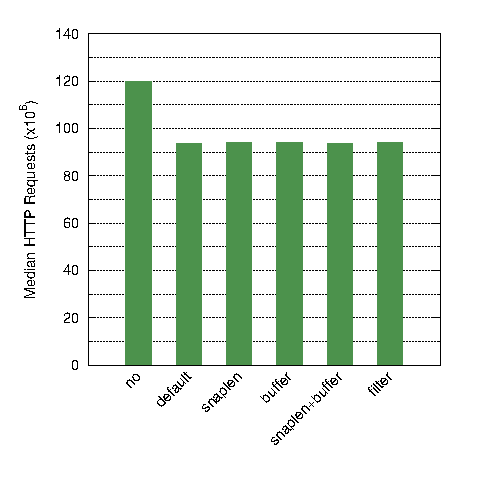
\includegraphics[width=0.5\textwidth]{images/requests}
    \caption{Anzahl der von wrk gesendeten HTTP Requests}\label{fig:results}
\end{figure}

Wie in Abbildung~\ref{fig:results} zu erkennen ist nimmt die Anzahl der
gesendeten HTTP Requests von wrk stark ab sobald tcpdump parallel zum Webserver
betrieben wird. Dabei kommt es zu eine Reduzierung der Requests um circa 25~\%
von rund 120 Million auf rund 90 Million Requests. Dies kann durch die erhöhte
Last auf dem ib6 Server erklärt werden. Zum einen werden nun alle Requests von
zwei Sockets verarbeiten. Außerdem teilen sich der Webserver und tcpdump nun
die verfügbaren Rechenkapazität auf dem Server. Weiterhin ist zu erkennen,
dass dieser Einfluss nahe zu konstant für alle Messungen mit tcpdump ist.

\begin{figure}
  \begin{subfigure}[b]{0.5\textwidth}
    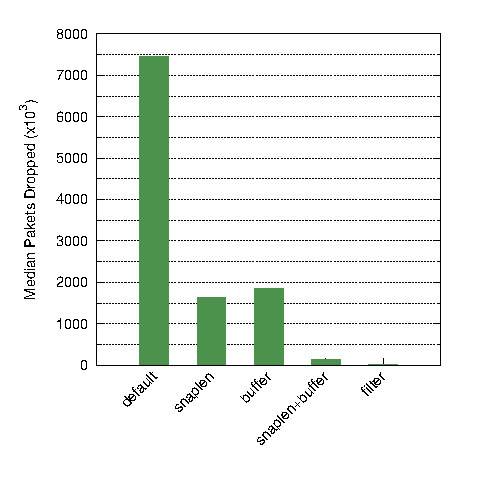
\includegraphics[width=\textwidth]{images/dropped}
    \caption{Anzahl der Pakete die vor tcpdump verloren wurden}\label{fig:dropped}
  \end{subfigure}
  %
  \begin{subfigure}[b]{0.5\textwidth}
    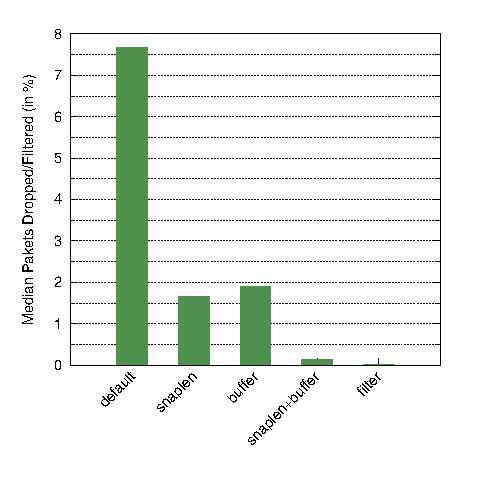
\includegraphics[width=\textwidth]{images/dropped-percentage}
    \caption{Prozentuale Anzahl der Pakete die vor tcpdump verloren wurden}\label{fig:dropped-percentage}
  \end{subfigure}
\caption{Paketverlust bevor tcpdump die Pakete auswerten konnte}\label{fig:results}
\end{figure}

In Abbildung~\ref{fig:dropped} ist die Anzahl der von tcpdump verloren Pakete
gezeigt. Zusätzlich zeigt~\ref{fig:dropped-percentage} den prozentualen Anteil
der verloren Paket von den empfangen Paketen.  Es zeigt sich das der
Paketverlust im Szenario \texttt{default} am Höchsten ist. Und das durch die
Anpassung der tcpdump Parameter eine starke Verbesserung erzielt werden kann.
Es scheint das die Reduzierung der aufgezeichneten Paketgröße einen größeren
Einfluss hat als eine Erhöhung des Empfangsbuffers. Dies kann dadurch erklärt
werden, dass die Paketgröße sehr stark reduziert wurde, von 65535 auf 142
Bytes. Zwar wurden keine Pakete versendet, welche 65535 Bytes groß sind,
allerdings entscheidet diese Größe wie libpcap den Ring Empfangsbuffer
aufteilt. Dabei geht es von der größt möglichsten Paketgröße aus. Mit einer
geringen Paketgrößte kann somit der vorhanden Buffer besser genutzt werden.
Die Kombination der beiden Parameter führte zu eine Reduzierung der verloren
Pakete von rund 98~\% im Vergleich zu dem \texttt{default} Szenario. So wurden
im Szenario \texttt{snaplen+buffer} nur noch 0.145~\% der empfangen Paket
verloren. Im Letzten Szenario \texttt{filter} konnte noch einmal eine
Verbesserung durch den optimierten Filter erzielt werden, hierbei sank die Zahl
der verloren Pakete auf 0.004~\%. Somit konnten fast alle Pakete bei einer Last
von rund 300.000 Requests pro Sekunde aufgezeichnet werden.
